\documentclass{article} 
\usepackage{amsmath} 
\usepackage{amssymb} 
\usepackage{amsthm} 
\usepackage[margin=0.2in]{geometry} 
\usepackage{hyperref} 
\usepackage{physics} 
\usepackage{tikz} 
\usepackage{mathtools}
\mathtoolsset{showonlyrefs} 
\theoremstyle{definition} 
\newtheorem{theorem}{Theorem}[section] 
\newtheorem{corollary}{Corollary}[theorem] 
\newtheorem{lemma}[theorem]{Lemma} 
\newtheorem{definition}{Definition}[section] 

\author{Connor Duncan}
\date{\today}

\title{notes-09-20-2019}
\begin{document}
\abstract{A single document copy of these notes, as well as a mirror of every note, can be found at \url{connorduncan.xyz/notes}}
\subsection{Electrons in metallic solids} Not really such a thing as a free electron. Mostly, we have atoms in a lattice. Let's start with a 1-d situation \begin{center} 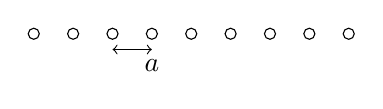
\begin{tikzpicture} \foreach \x in {-2,-1.5,...,2}{ \draw (\x,0) circle (2pt); } \draw[<->] (-1,-0.2) -- (-0.5,-0.2) node[anchor=north]{$a$}; \end{tikzpicture} \end{center} We can write down $\ket{n}$, the state of $e^-$ sitting on an atom $n$, which gives $\bra{n}\ket{m}=\delta_{nm}$. We can write down the hamiltonian as $H_0$, the usual, and some $H_1$ to account for the dynamics, where the electrons are only allowed to move between neighbors. \begin{align} H_0=E_0\sum_N\ket{n}\bra{n} && H_1=-t\sum_N\ket{n}\bra{n+1}+\ket{n+1}\bra{n} \end{align} We just want to find eigenstates of this now, by putting this into Schroedingers equation and solving the eigenvalue equation, which gives us \begin{equation} E_0\sum_M\psi_m\ket{m}-t\sum_m\psi_{m+1}\ket{m}+\psi_m\ket{m+1}=E\sum_m\psi_m\ket{m} \end{equation} Let's inner product on another state $n$, which gives us a set of equations for another state $n$, this gives us an equation \begin{equation} E_o\psi_n-t(\psi_{n+1}+\psi_{n-1})=E\psi_n \end{equation} We can solve this to get \begin{equation} \psi_n=\frac{e^{ikna}}{\sqrt{N}} \end{equation} If we take the symmetry $k\rightarrow k+\frac{2\pi}{a}$, then we only need to look at $k\in\left[\frac{-\pi}{a},\frac{\pi}{a}\right]$. This is actually just the \textbf{Brilloun Zone} of the lattice. $k$ comes in a discrete unit, $\frac{2\pi}{aN}$. This allows the counting of the basis. We can get this out by just enforcing periodic boundary conditions on $k$. This spits out \begin{equation} E=E_0-2t\cos ka \end{equation} We can plot this as \begin{center} \begin{tikzpicture}[scale=3] \draw[->] (0,0)--(1,0); \draw[->] (0,0)--(0,1); \draw plot[domain=-200:200,variable=\x,smooth] ({(\x+90)/360},{-.5*cos(\x)+0.5}); \end{tikzpicture} \end{center} \paragraph{Remarks} \begin{enumerate} \item For arbitrary small perturbations, the hopping wavefunction (pos space) completely delocalized. \item All of original degeneracy has been lifted \item For small $|k|\ll\frac{\pi}{a}$, we have $E_k\approx\frac{\hbar^2k^2}{2m^*}$, with $m^*=\frac{\hbar^2}{2a^2t}$. \end{enumerate} This $m^*$ can be tought of as a sort of renormalized mass that comes from the interaction with the lattice, but leaves our wavefunction completelet delocalized, as we expect. \subsubsection{More Realistic Treatment} Assume $e^{-}$ can move anywhere along $\hat x$, but assume there's some weak periodic potential $V(x)=V(x+a)$. The hamiltonian is just \begin{equation} H=\frac{p^2}{2m}+V(x) \end{equation} Bare energies of the problem can be obtained by taking the fourier transform, and getting \begin{equation} E_0(k)=\frac{\hbar^2k^2}{2m} \end{equation} We probably should do perturbation theory. Naively, it looks as if since for $\pm k$, $E_o(\pm k)$ is the same, we should do degenerate perurbation theory. We can just get a new basis expressed as linear combinations of $\ket{\pm k}$. We should always check, however, that \begin{equation} \bra{k}V\ket{k'}\neq 0 \end{equation} Since we know that $V$ is periodic, we can re-expand our perturbation $V$ in the fourier basis. Let's expand $V$ as \begin{equation} V(x)=\sum_n V_ne^{2\pi nx/a} \end{equation} with \begin{equation} V_n=\frac{1}{a}\int_0^adxV(x)e^{-2\pi inx/a} \end{equation} We can combine this all to get \begin{equation} \bra{k}V\ket{k'}=\int dx\sum_nV_ne^{i\left(k-k'+\frac{2\pi n}{a}\right)x} =\sum_n V_n\mathrm{\delta}\left(k'-k+\frac{2\pi n}{a}\right) \end{equation} Momenta $k,k'$ have to match $\frac{2\pi n}{a}$ in order for the $V$ to have an effect. That is to say, that mixing occurs as \begin{equation} k=k'+\frac{2\pi n}{a} \end{equation} Now, we apply the condition to our degenerate states \begin{center} 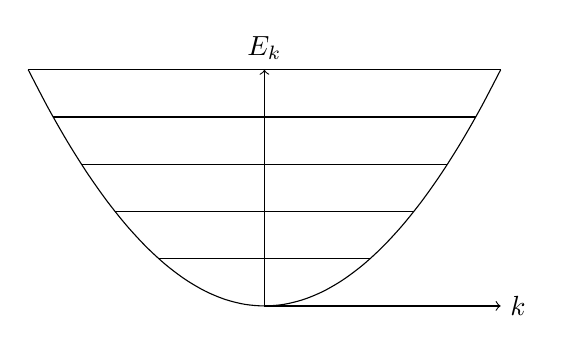
\begin{tikzpicture}[scale=3] \draw[->] (0,0)--(1,0) node[anchor=west]{$k$}; \draw[->] (0,0)--(0,1) node[anchor=south]{$E_k$}; \draw plot[domain=-1:1,variable=\x,smooth] ({\x},{\x*\x}); \foreach \x in {0,0.2,...,1}{ \draw ({-sqrt(\x)},{\x})--({sqrt(\x)},{\x}); } \end{tikzpicture} \end{center} This is another way of thinking about the emergence of the Brillouin Zone. It's just the first place a periodic perturbation mixes a $\ket{\pm k}$ state. We can consider some basic limits of this. \paragraph{Case 1: Low momenta}For low momenta, $|k|\ll\frac{\pi}{2a}$. \begin{equation} E(k)=\frac{\hbar^2 k^2}{2m}+\bra{k}V\ket{k}+\sum_{k=k'}\frac{|\bra{k}V\ket{k'}|^2}{E_0(k)-E_0(k')}+\dots \end{equation} but the perturbation is small, so it should behave like a free particle. \paragraph{Case 2: At Edge of Brillouin Zone}
\end{document}
